\documentclass[10pt,twocolumn,letterpaper]{article}

\usepackage[review]{cvpr}

% Additional packages for Special-SAM paper
\usepackage{amsmath}
\usepackage{amssymb}
\usepackage{booktabs}
\usepackage{multirow}
\usepackage{capt-of}
\usepackage{enumitem}


\definecolor{cvprblue}{rgb}{0.21,0.49,0.74}
\usepackage[pagebackref,breaklinks,colorlinks,allcolors=cvprblue]{hyperref}

\def\paperID{*****}
\def\confName{CVPR}
\def\confYear{2026}

\title{Where Do Visual Concepts Break Down? Decoder-Only Adaptation of SAM for Camouflaged Segmentation}
\author{Anonymous CVPR submission\\Paper ID \paperID}

\begin{document}
\maketitle

\begin{abstract}
SAM's ViT-H encoder, pre-trained on over one billion masks, learns rich visual representations---but its decoder fails to map these representations to correct masks when objects are camouflaged. We isolate this failure by freezing the encoder and fine-tuning only the 4M-parameter mask decoder on COD10K. This raises mIoU from 57.2\% to 73.8\% and reduces prompt sensitivity from 3.5$\times$ to 1.1$\times$ across four prompt types. The decoder generalizes without retraining: +18.8 mIoU on CAMO and +18.5 on NC4K. These results suggest that SAM's encoder already captures visual concepts relevant to camouflage---texture gradients, subtle edge patterns---but the general-purpose decoder does not convert them into boundary decisions. Camouflage thus serves as a diagnostic setting that reveals where concept utilization, rather than concept representation, is the bottleneck in foundation segmentation models.
\end{abstract}

\section{Introduction}

Foundation models for segmentation learn visual concepts---object boundaries, texture transitions, spatial structure---from massive datasets. SAM~\cite{kirillov2023sam}, trained on over one billion masks, segments almost anything. Yet camouflaged objects expose a striking failure: on COD10K~\cite{fan2020cod10k}, SAM ViT-H achieves only 57.2\% mIoU with center-of-mass prompts and 20.5\% with edge prompts (\cref{tab:main_viscon}). Camouflaged organisms have evolved to defeat visual detection, and SAM's general-purpose decoder has never learned to interpret subtle texture disruptions as boundaries.

This failure raises a question about visual concept representation: does the encoder lack the relevant concepts, or does the decoder fail to use them? If SAM's ViT-H encoder, pre-trained on 11M images, already captures the low-level texture gradients that distinguish camouflaged foreground from background, then specializing only the decoder should recover substantial performance. That is what we observe.

Prior SAM adaptation methods typically modify the encoder via adapters~\cite{chen2023samadapter}, redesign prompt pathways~\cite{hao2024comprompter}, or add dual-stream modules~\cite{liu2025dualstream}. These approaches improve performance but conflate two questions: whether the encoder needs better features, and whether the decoder needs better feature utilization. By changing only the decoder, we isolate the latter.

Our strongest evidence is not the average gain alone, but the change in behavior across prompts. Decoder specialization sharply reduces prompt sensitivity (\cref{tab:main_viscon}), and an ablation confirms this is learned: mixed point/box training consistently outperforms point-only and box-only alternatives (\cref{tab:prompt_ablation_viscon}). The specialized decoder also generalizes to held-out camouflage datasets (CAMO, NC4K) without retraining, suggesting it learns transferable camouflage concepts rather than dataset-specific patterns.

\noindent\textbf{Contributions.}
\begin{enumerate}
    \item We show that decoder-only adaptation yields +16.6 mIoU on COD10K with no architecture changes, 90-minute training, and a 16MB checkpoint---evidence that SAM's encoder already represents camouflage-relevant visual concepts.
    \item We demonstrate prompt robustness: mixed-prompt training reduces sensitivity from 3.5$\times$ to 1.1$\times$, and the gain transfers to held-out datasets (+18.8 mIoU on CAMO, +18.5 on NC4K).
    \item We provide a diagnostic lens: camouflage as a setting that separates concept representation (encoder) from concept utilization (decoder) in foundation segmentation models.
\end{enumerate}

\section{Related Work}

\noindent\textbf{Camouflaged object detection.}
Dedicated COD architectures---SINet~\cite{fan2020cod10k}, ZoomNet~\cite{pang2022zoomnet}, SegMaR~\cite{jia2022segmar}---design task-specific networks from scratch. We instead leverage SAM's pre-trained representations and ask how far decoder-only adaptation can go without domain-specific architecture.

\noindent\textbf{SAM adaptation.}
SAM-Adapter~\cite{chen2023samadapter} injects learnable modules inside the encoder, COMPrompter~\cite{hao2024comprompter} redesigns the prompt pathway, and Liu~\etal~\cite{liu2025dualstream} add dual-stream adapters. All modify the encoder, conflating feature quality with feature utilization. We fine-tune only the existing decoder, isolating the utilization question.

\noindent\textbf{Parameter-efficient fine-tuning.}
LoRA~\cite{hu2022lora} and prompt tuning~\cite{lester2021prompt} adapt large models by adding small parameter sets to the encoder or prompt pathway. Our approach is simpler: we add zero new parameters and train only the existing 4M-parameter mask decoder.

\section{Method}
SAM consists of a ViT-H image encoder ($\sim$632M parameters), a prompt encoder, and a mask decoder ($\sim$4M parameters). We freeze the image encoder and prompt encoder, and train only the mask decoder (\cref{fig:architecture}).

\noindent\textbf{Pre-computed embeddings.} We run the frozen encoder once on all training images and cache embeddings as \texttt{.npy} files, eliminating the encoder forward pass from training.

\noindent\textbf{Mixed-prompt training.} Each iteration randomly selects between a point prompt (random foreground pixel) and a bounding box prompt (tight GT box) with 50/50 probability. This prevents the decoder from overfitting to any single prompt type and provides a direct test of whether gains transfer across prompt styles.

\noindent\textbf{Loss and optimization.} We minimize $\mathcal{L} = 0.5 \cdot \mathcal{L}_{\text{BCE}} + 0.5 \cdot \mathcal{L}_{\text{Dice}}$, where BCE enforces pixel-level boundaries and Dice maintains region-level coherence. We use AdamW (lr $10^{-4}$, cosine schedule, 1-epoch warmup, 15 epochs). Training takes $\sim$90 minutes on a single A100 with pre-computed embeddings.

\noindent\textbf{Evaluation protocol.} We evaluate four prompt strategies of increasing difficulty: \textbf{Center-of-Mass} (1pt), \textbf{Edge} (1pt on boundary contour), \textbf{Multi-Grid} (4pt), and \textbf{Multi-Random} (3pt). Following SAM's standard protocol~\cite{kirillov2023sam}, prompts are derived from ground-truth masks to simulate idealized user clicks. We report mIoU on the full 2,026-image COD10K camouflaged test set, as well as on CAMO (250 images) and NC4K (4,121 images) for cross-dataset evaluation.

\begin{figure}[t]
    \centering
    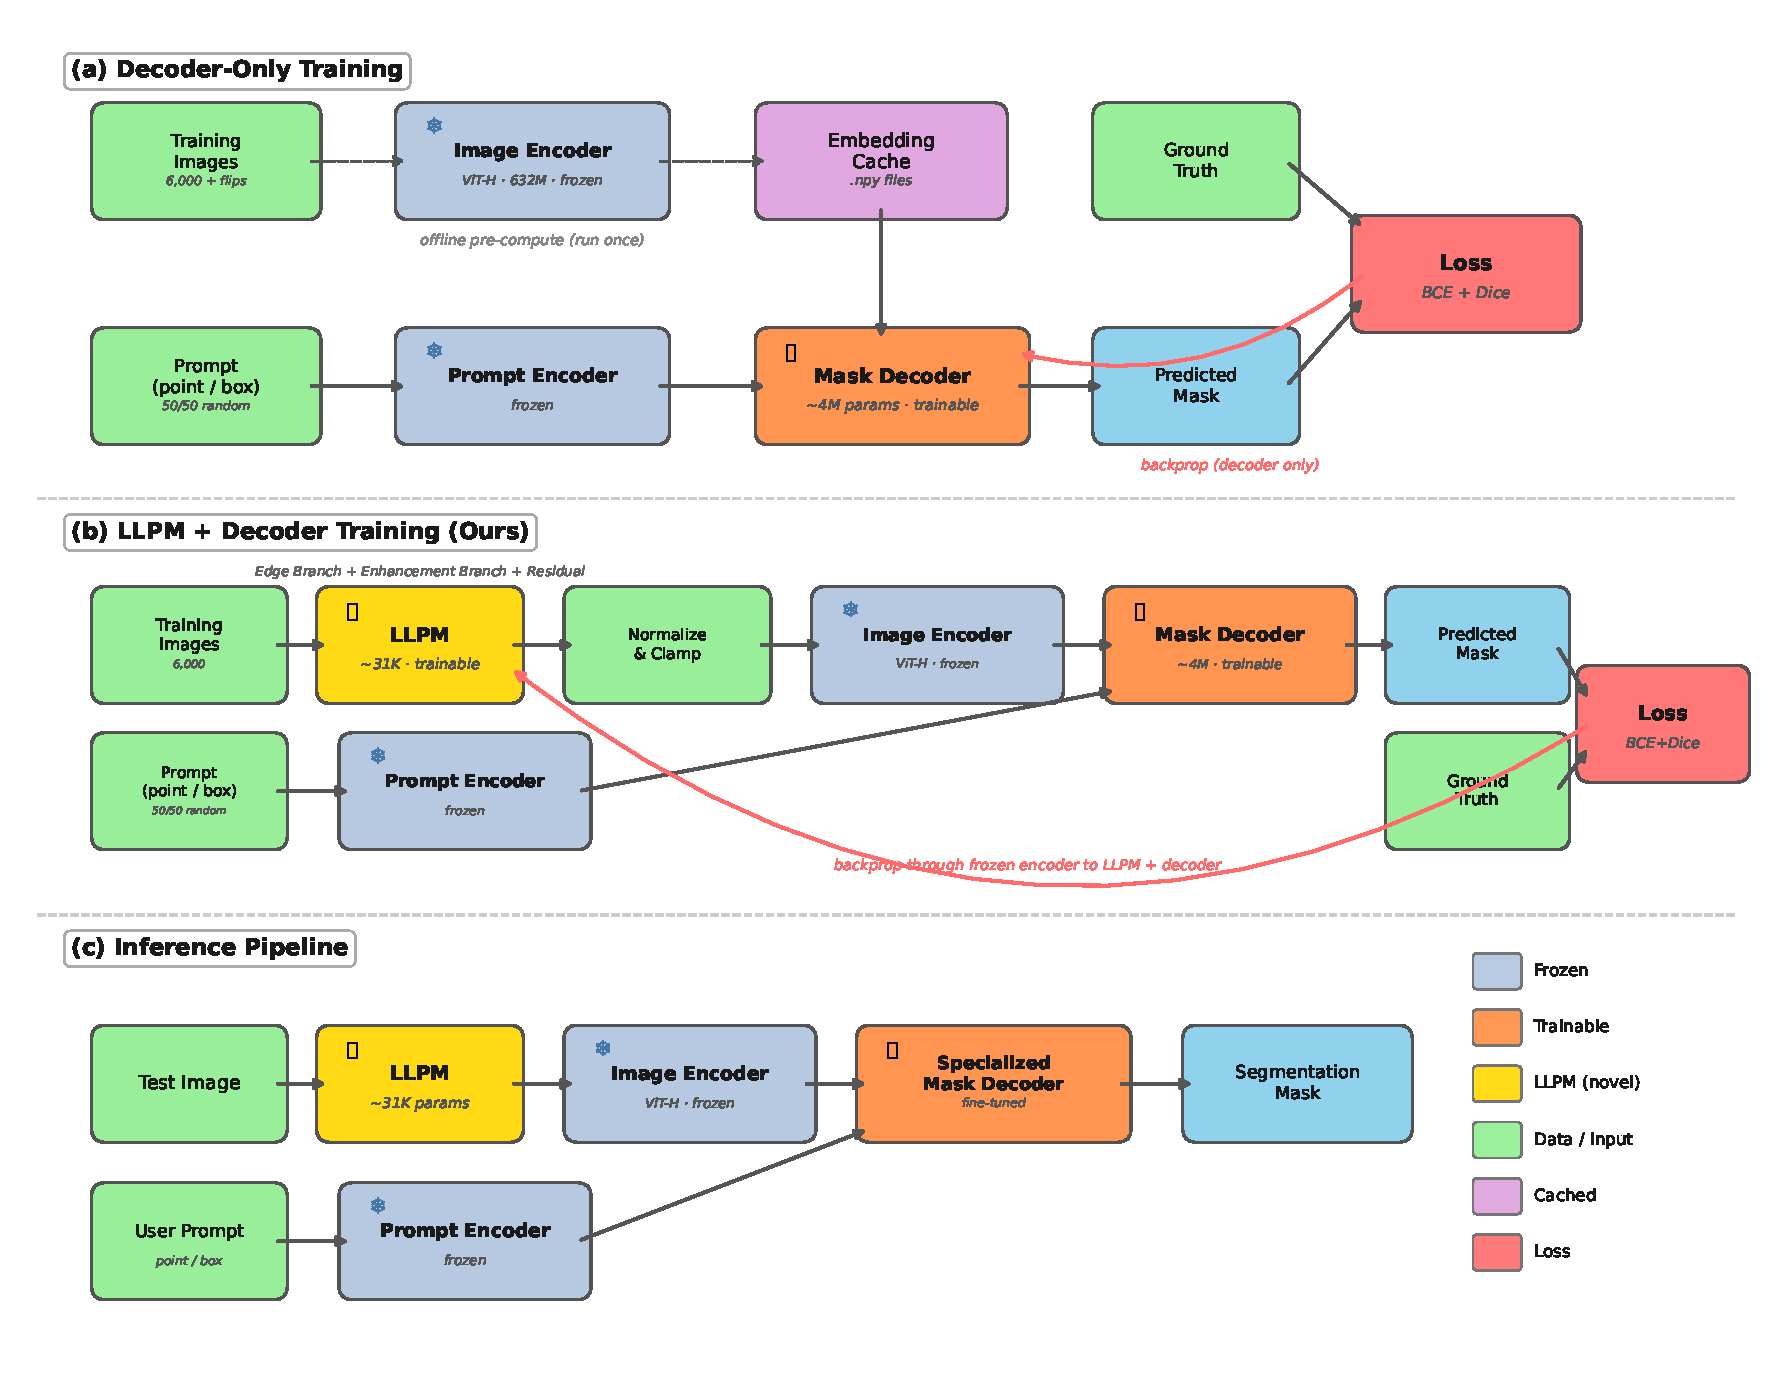
\includegraphics[width=\columnwidth]{figures/architecture_diagram.pdf}
    \caption{\textbf{Decoder-only specialization of SAM.} We freeze the ViT-H image encoder and prompt encoder, cache image embeddings, and fine-tune only the 4M-parameter mask decoder with mixed point/box prompts.}
    \label{fig:architecture}
\end{figure}

\section{Results}

\subsection{Decoder Adaptation Improves All Prompt Types}

\begin{table}[t]
\centering
\caption{\textbf{Main results on COD10K} (2,026 test images). Decoder-only adaptation improves all prompt strategies and sharply reduces prompt sensitivity.}
\label{tab:main_viscon}
\small
\begin{tabular}{lcccc}
\toprule
Prompt & Base & Ours & $\Delta$ & Rel.~$\Delta$ \\
\midrule
Center-of-Mass & 0.572 & 0.738 & +0.166 & +28.9\% \\
Edge & 0.205 & 0.694 & +0.489 & +238.1\% \\
Multi-Grid & 0.682 & 0.756 & +0.074 & +10.9\% \\
Multi-Random & 0.727 & 0.776 & +0.049 & +6.7\% \\
\midrule
\textit{Range} & \textit{3.5$\times$} & \textit{1.1$\times$} & & \\
\bottomrule
\end{tabular}
\end{table}

\Cref{tab:main_viscon} shows that freezing the encoder and adapting only the decoder improves every prompt strategy. The largest gain is on edge prompts (+238\% relative), the setting where subtle boundary interpretation matters most. Base SAM's mIoU varies 3.5$\times$ across prompt types (0.205 to 0.727); the specialized decoder varies only 1.1$\times$ (0.694 to 0.776). The straightforward reading is that visual information useful for camouflage is already present in the frozen representation, but the default decoder does not convert it into reliable boundary decisions.

\subsection{Prompt Robustness Is Learned, Not Accidental}

\begin{table}[t]
\centering
\caption{\textbf{Prompt-mix ablation} (COD10K, 2,026 test images). Mixed training produces the most robust decoder; box-only collapses on point prompts.}
\label{tab:prompt_ablation_viscon}
\small
\begin{tabular}{lcccc}
\toprule
\multirow{2}{*}{Training} & \multicolumn{4}{c}{Test Prompt mIoU} \\
\cmidrule(lr){2-5}
 & CoM & Edge & Grid & Random \\
\midrule
Point-only & .699 & .672 & .725 & .768 \\
Box-only & .376 & .501 & .389 & .455 \\
\textbf{Mixed (ours)} & \textbf{.738} & \textbf{.694} & \textbf{.756} & \textbf{.774} \\
\bottomrule
\end{tabular}
\end{table}

\Cref{tab:prompt_ablation_viscon} validates that prompt robustness arises from mixed training, not from fine-tuning alone. Mixed-prompt training outperforms point-only on all test strategies (by 2--4 mIoU) and box-only by 19--37 mIoU. Box-only training collapses catastrophically on point prompts (0.376 CoM), confirming that robustness requires explicit multi-modal prompt exposure. By alternating point and box prompts, the decoder learns \emph{what} the camouflaged object is rather than \emph{where the user clicked}---a more concept-grounded mapping from features to masks.

\subsection{Cross-Dataset Generalization}

\begin{table}[t]
\centering
\caption{\textbf{Cross-dataset generalization} (Center-of-Mass prompt, with multi-prompt mIoU range). The decoder is trained only on COD10K and evaluated on held-out datasets without retraining. \textit{Range} reports the max/min mIoU ratio across all four prompt types.}
\label{tab:crossdataset}
\small
\begin{tabular}{llcccc}
\toprule
Dataset & Model & mIoU & $S_\alpha$ & $E_\phi$ & MAE$\downarrow$ \\
\midrule
\multirow{2}{*}{CAMO (250)} & Base SAM & .489 & .672 & .748 & .122 \\
 & Ours & \textbf{.677} & \textbf{.797} & \textbf{.887} & \textbf{.073} \\
\midrule
\multirow{2}{*}{NC4K (4,121)} & Base SAM & .567 & .728 & .805 & .093 \\
 & Ours & \textbf{.752} & \textbf{.848} & \textbf{.929} & \textbf{.045} \\
\bottomrule
\end{tabular}
\end{table}

% TODO: After running eval_crossdataset.sh with all four prompt types,
% add a Range row to this table (e.g., CAMO Range: Base X.Xx / Ours 1.Xx)
% and update the prose below with the actual cross-dataset range values.

A critical test of whether the decoder learns generalizable visual concepts or dataset-specific shortcuts is cross-dataset transfer. \Cref{tab:crossdataset} shows that the decoder, trained exclusively on COD10K, generalizes consistently: +18.8 mIoU on CAMO and +18.5 on NC4K without any retraining. This confirms that decoder specialization learns transferable camouflage cues---the ability to map subtle texture and boundary evidence to object masks---rather than memorizing COD10K-specific patterns.

\subsection{Context: Comparison with Existing Methods}

\begin{table}[t]
\centering
\caption{\textbf{Landscape comparison} on COD10K. Dedicated COD methods are fully automatic; SAM-based methods use encoder/prompt tuning; ours uses oracle prompts.\textsuperscript{$\dagger$} These are \emph{not} head-to-head comparisons.}
\label{tab:comparison}
\small
\resizebox{\columnwidth}{!}{%
\begin{tabular}{llcccc}
\toprule
Method & Type & $S_\alpha$ & $E_\phi$ & $F_\beta^w$ & MAE$\downarrow$ \\
\midrule
SINet~\cite{fan2020cod10k} & Auto & .776 & .864 & .631 & .043 \\
ZoomNet~\cite{pang2022zoomnet} & Auto & .838 & .911 & .729 & .029 \\
SAM-Adpt.~\cite{chen2023samadapter} & Enc.\ adapt & .883 & .918 & .801 & .025 \\
COMPr.~\cite{hao2024comprompter} & Prompt adapt & .889 & .949 & .821 & .023 \\
\midrule
\textbf{Ours} (Grid)\textsuperscript{$\dagger$} & Dec.\ only & .861 & .951 & .841 & .024 \\
\bottomrule
\end{tabular}}
\vspace{1pt}
{\footnotesize \textsuperscript{$\dagger$}Oracle prompts from GT masks. Not comparable to fully automatic methods.}
\end{table}

\Cref{tab:comparison} contextualizes decoder-only adaptation within the broader COD landscape. Under oracle prompts, our method achieves competitive $E_\phi$ and $F_\beta^w$ but lower $S_\alpha$ than encoder-adaptation methods (SAM-Adapter, COMPrompter). This is consistent with our conclusion: encoder and decoder specialization address complementary aspects of the problem. Decoder-only adaptation recovers substantial performance with no new parameters and 90-minute training, but does not replace encoder-side adaptation.

\begin{figure*}[t]
    \centering
    \includegraphics[width=\textwidth]{figures/qualitative_comparison.png}
    \caption{\textbf{Qualitative comparison} (center-of-mass prompts). Each row: input image, ground-truth mask, base SAM prediction, our decoder-only prediction. Base SAM frequently segments only the most salient region near the prompt, missing large portions of camouflaged objects. The specialized decoder follows true object boundaries even when coloration matches the background.}
    \label{fig:qualitative}
\end{figure*}

\section{Discussion}

\noindent\textbf{What this reveals about visual concept representation.}
Our results contribute to understanding how foundation models organize visual concepts. SAM's ViT-H encoder, pre-trained on 1B+ masks, appears to already capture texture gradients and edge patterns relevant to camouflage. The decoder---trained on general segmentation---has not learned that \emph{subtle} texture disruptions signify boundaries. The substantial mIoU gains from training only 0.6\% of parameters (\cref{tab:main_viscon}) suggest that, at least for camouflage, the bottleneck lies in concept utilization (decoder) rather than concept representation (encoder). Camouflage serves as a useful diagnostic because it isolates a regime where the gap between having a concept and acting on it is unusually large.

\noindent\textbf{Prompt robustness as concept grounding.}
The sharp reduction in prompt sensitivity (\cref{tab:main_viscon}) suggests that mixed-prompt training produces a decoder grounded in the visual concept of the object rather than in prompt-specific heuristics. Point-only training overfits to spatial proximity; box-only training overfits to box geometry (\cref{tab:prompt_ablation_viscon}). Mixed training forces the decoder to understand object structure, which is why improvement transfers to prompt types never seen during training.

\noindent\textbf{Complementary directions.}
As a preliminary extension, we tested a Learnable Local Preprocessing Module (LLPM, $\sim$31K parameters) placed before the frozen encoder. LLPM consists of two branches---an edge-attention branch (Conv $3{\to}32{\to}1$, sigmoid) and a channel-enhancement branch (grouped convs $3{\to}64{\to}3$)---fused via a learnable scalar gate $\alpha$ (initialized at 0.1, converging to $\sim$0.185). Because gradients must flow through the frozen encoder to reach LLPM, training requires live encoder forward passes ($\sim$7.5 hours vs.\ 90 minutes for decoder-only). This module yields a further +2.5 mIoU on edge prompts by enhancing boundary signals in input space, suggesting that pre-encoder and decoder-side adaptation are complementary. Encoder-adaptation methods~\cite{chen2023samadapter,hao2024comprompter} achieve higher absolute $S_\alpha$, confirming that encoder specialization also remains important. A practical system may benefit from both, and pairing our decoder with an automatic prompt generator is a natural next step toward fully automatic deployment.

\noindent\textbf{Limitations.}
(1)~Our evaluation uses oracle GT-derived prompts following SAM's standard protocol; deployment requires a prompt source.
(2)~Results are from single training runs without confidence intervals.

{\small
\bibliographystyle{ieeenat_fullname}
\bibliography{main}
}

\end{document}
